\chapter{Vertices and Transforms}

\begin{figure}[htb]\centering
  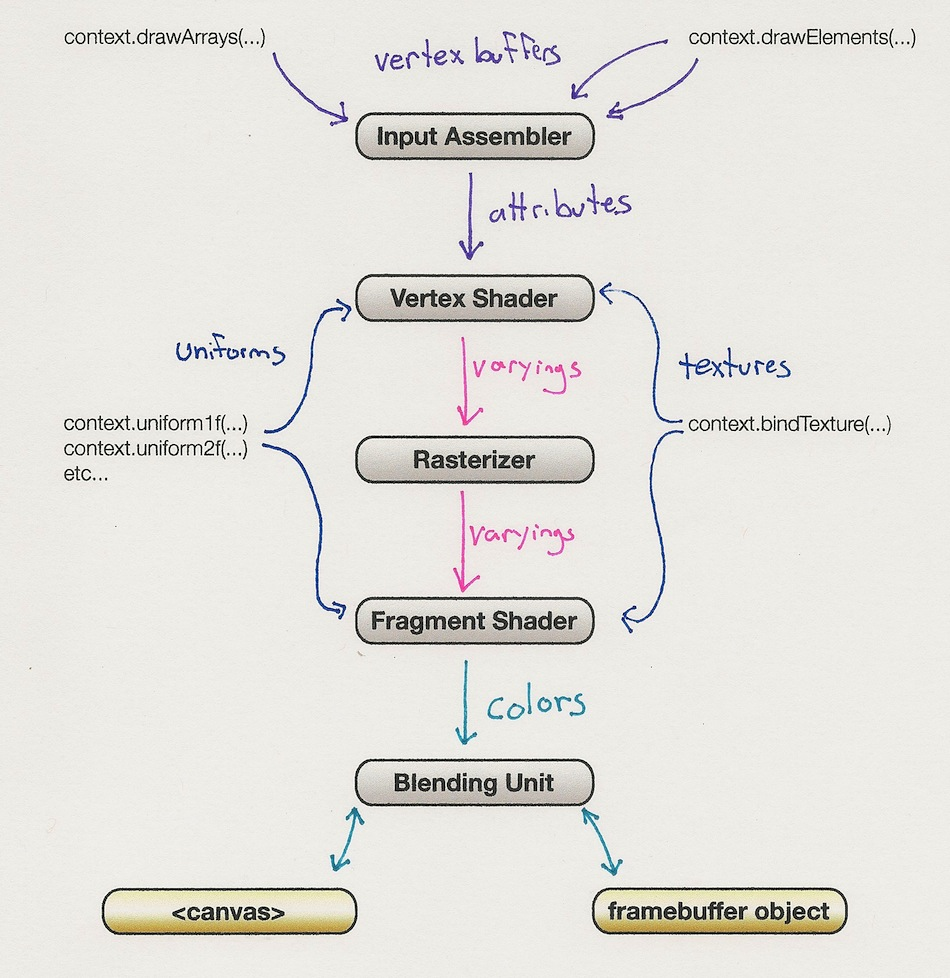
\includegraphics[width=70mm]{pipeline.jpg}
  \caption{High level view of the WebGL / OpenGL ES pipeline}
  \label{fig:AssemblyLine}
\end{figure}

\section{WebGL at 10,000 feet}
\summary{High-level overview of the WebGL rendering pipeline.}

Earlier we mentioned that only two WebGL functions that can actually render 3D geometry: \code{drawArrays} and \code{drawElements}.  Both of these simply push a set of \index{vertices} vertices into the WebGL pipeline.  The vertices become rasterized into \index{fragments} \term{fragments}, or pixel values in the canvas.  Every vertex is defined by a set of \term{vertex attributes}, one of which is usually an XYZ coordinate.  Vertices come together to form \term{primitives}, which include point sprites, lines, and triangles.

Vertices initially belong to a swath of memory called a \term{vertex buffer}, and WebGL provides a rich API that allows you to specify how heterogenous attributes can be packed into a vertex buffer.  Figure~\ref{fig:AssemblyLine} depicts how vertex data flows through the pipeline, starting off in vertex buffers, eventually transforming into pixels in the canvas.

Two phases of this data flow are programmable: the vertex shader and the fragment shader.  Shaders are bundled together into \index{program object} \term{program objects}.   More precisely, a program object is the linked combination of a compiled vertex shader, a compiled fragment shader, a set of bindings for constant inputs (\term{uniforms}), and a set of bindings for vertex-varying inputs (\term{attributes}).

We'll dive deeper into shaders and vertex buffers later in this chapter; for now, see Listing~\ref{lst:Taste} for a taste of the various set-up that must be performed before actually pushing the vertices into the pipeline.

\begin{lstlisting}[
    caption={The typical state-setting that occurs before \code{drawArrays}.},
    escapechar=\%,
    label=lst:Taste,
    language=JavaScript]
// Bind a program object and set up a couple uniforms.
gl.useProgram(program);
gl.uniform1f(program, shininess, 0.5);
gl.uniform4fv(program, color, [1,1,0,1]);

// Bind a vertex buffer and set up the position attribute.
gl.bindBuffer(gl.ARRAY_BUFFER, buffer);
gl.enableVertexAttribArray(attribs.POSITION);
gl.vertexAttribPointer(attribs.POSITION, 3, gl.FLOAT, false, 0, 0);

// Finally, draw two triangles (six vertices), starting at vertex 0.
gl.drawArrays(gl.TRIANGLES, 0, 6);
\end{lstlisting}

\section{Vector Algebra with JavaScript}
\notetoself{This sections walks through giza's implementation of vector and matrix classes.  Rotation, translation, and scale are given a very brief treatment.}

\section{The Typical Life of a Vertex}
\notetoself{Describes model, view, and projection transforms.}

\section{Shading Language Basics}
\notetoself{Explains uniforms, attributes, and varyings.  Walks through trivial \texttt{main} functions for vertex and fragment shaders.}

\section{Program Objects}

\subsection{Fetching and Compiling Shader Strings}

Shaders are specified with multi-line strings that get passed to WebGL for compilation.  There are several ways to embed a multi-line string in JavaScript code: you can end each line with a backslash, or concatenate a series of single-line strings with the \code{+} operator, or create an array of strings that become glued together with \code{join}.

None of embedded options are ideal, so another idea is to download the entire shader from an external file.  With jQuery, this is easily accomplished with \code{\$.get}.

In this book's sample code however, we've decided to use the HTML file as a container for all shader strings by authoring the shaders inside \code{<script>} elements.  Embedding arbitrary strings in \code{<script>} is also a common practice with templating systems such as \mbox{\code{handlebars.js}}.

Listing~\ref{lst:embed} shows how we embed a fragment shader in HTML.

\begin{lstlisting}[
    language=HTML,
    caption={Embedding a shader string in HTML.},
    label=lst:embed]
<script id="simplefs" type="x-shader/x-fragment">
  precision highp float;
  varying vec3 vColor;
  void main() {
      gl_FragColor = vec4(vColor, 1.0);
  }
</script>
\end{lstlisting}

With this system, every shader string is assigned a unique identifier in its enclosing script tag.  The string can then easily be retrieved using jQuery:

\begin{lstlisting}[language=JavaScript]
var fsText = $('#simplefs').text();
\end{lstlisting} % $

Alternatively, you can fetch the string through the raw DOM element:

\begin{lstlisting}[language=JavaScript]
var fsText = document.getElementById('simplefs').innerHTML;
\end{lstlisting}

After obtaining a shader string, the next step is to pass it into a WebGL shader object and compile it:

\begin{lstlisting}[language=JavaScript]
var fsObject = gl.createShader(gl.FRAGMENT_SHADER);
gl.shaderSource(shaderObject, fsText);
gl.compileShader(fsObject);
var status = gl.getShaderParameter(fsObject, gl.COMPILE_STATUS);
if (!status) {
 console.error(gl.getShaderInfoLog(fsObject));
}
\end{lstlisting}

Since GLSL does not have a \code{\#include} statement, it's often useful to stitch together several strings to form a single shader.  This allows you to share a single function (or block of uniforms) among several shader objects.  See Listing~\ref{lst:GIZA:compileShader} for Giza's implementation of a utility function that takes a list of ids and a shader type.  It fetches the strings from the DOM, glues them together, and compiles them.

\begin{lstlisting}[
    language=JavaScript,
    caption={The \code{compileShader} function (error checking omitted).},
    label=lst:GIZA:compileShader]
GIZA.compileShader = function(ids, type) {
  var gl = GIZA.context;
  var sourceText = "";
  for (var i = 0; i < ids.length; i++) {
    sourceText += document.getElementById(id).innerHTML;
  }
  var shaderObject = gl.createShader(type);
  gl.shaderSource(shaderObject, sourceText);
  gl.compileShader(shaderObject);
  return shaderObject;
};
\end{lstlisting}

\subsection{Creating Program Objects}

Recall that a \index{program object} program object is the linked combination of a compiled vertex shader, a compiled fragment shader, and a set of bindings for uniforms and attributes.

Giza provides a utility function that takes two id lists (one for the vertex shader, one for the fragment shader), aggregates them, compiles them, and links them into a program object.  See Listing~\ref{lst:GIZA:compileProgram} for the skeletal implementation -- we'll flesh it out a bit in upcoming sections.

\begin{lstlisting}[
    language=JavaScript,
    caption={The \code{compileProgram} function (abridged).},
    label=lst:GIZA:compileProgram]
GIZA.compileProgram = function(vsIds, fsIds) {
  var gl = GIZA.context;
  var vShader = GIZA.compileShader(vsIds, gl.VERTEX_SHADER);
  var fShader = GIZA.compileShader(fsIds, gl.FRAGMENT_SHADER);
  var program = gl.createProgram();
  gl.attachShader(program, vShader);
  gl.attachShader(program, fShader);
  // bind attributes here...
  gl.linkProgram(program);
  var status = gl.getProgramParameter(program, gl.LINK_STATUS);
  if (!status) {
    console.error("Could not link " + vsIds + " with " + fsIds);
  }
  // query uniforms here...
}
\end{lstlisting}

\subsection{Binding Vertex Attributes}

WebGL needs to know how to correllate data elements in the vertex buffer with attributes in the vertex shader.  Each attribute that the vertex shader reads has an associated string name and an associated integer handle.  The integer handle is used when specifying the vertex buffer layout, as you'll see in \ref{sec:VBOs}.

WebGL and other OpenGL-based APIs provide two ways of associating attributes with integers: you can let WebGL make the association, or you can bind them explicitly.  To allow WebGL to make the association, just compile and link the program object as you normally would, then query for the integer handles afterwards like so:

\begin{lstlisting}
var handle = gl.getAttribLocation(programObject, "Position");
\end{lstlisting}

However, I generally try to avoid this strategy, preferring instead to bind attributes explicitly using WebGL's \code{bindAttribLocation} method:

\begin{lstlisting}
var handle = 3;
gl.bindAttribLocation(programObject, handle, "Position");
\end{lstlisting}

My usual approach is to specify a single, authoratative enumeration of all possible vertex attributes used in my application; this allows me to decouple vertex buffer layouts from shaders.  In other words, I can more easily mix and match vertex buffers with shaders.  This practice is known as \index{semantic binding} \term{semantic binding} in the OpenGL community.

For example, suppose your application uses two program objects: one that applies a texture, and another that performs lighting (both of which we'll learn about in future chapters).  The texturing program requires two attributes: positions and texture coordinates.  The lighting program requires positions and normal vectors.  With semantic binding, your application would define an object for the superset of these attributes:

\begin{lstlisting}
var attribs = {
  POSITION: 0,
  NORMAL: 1,
  TEXCOORD: 2
};
\end{lstlisting}

One gotcha with \code{bindAttribLocation} is that it needs to occur after shader compilation but before program linking.  See Listing~\ref{lst:GIZA:compileProgram2} for how we augmented Giza's \code{compileProgram} method to do this for you.  Notice that we added a third argument to the function declaration.

\begin{lstlisting}[
    language=JavaScript,
    caption={Adding attribute binding to \code{compileProgram}.},
    label=lst:GIZA:compileProgram2]
GIZA.compileProgram = function(vsIds, fsIds, attribs) {
  ...
  for (key in attribs) {
    gl.bindAttribLocation(program, attribs[key], key);
  }
  gl.linkProgram(program);
  ...
};
\end{lstlisting}

\subsection{Querying and Setting Uniforms}

\subsection{Giza's top-level \code{compile} utility}
\notetoself{Describes a useful abstraction of the WebGL program object.}

\section{Lines and Triangles}
\notetoself{Explains the various primitive types (e.g., \texttt{LINES}), \texttt{drawArrays}, and \texttt{drawElements}.}

\section{Typed Arrays and VBOs}
\label{sec:VBOs}

\notetoself{Shows how heterogeneous data (e.g., colors and positions) can be interleaved and submitted to WebGL.}

\subsection{GIZA.BufferView}

\rrecipe{Recipe 2: Color Wheel}
\notetoself{Spinning wheel with various colors at each vertex.}
